\section{Mikrofony}
\label{cha:mikrofony}

Wybór mikrofonu był największym problemem ze względu na różne technologie wykonania (elektretowy, MEMS) oraz dużo różnych parametrów. Początkowo miał to być mikrofon elektretowy, jednak okazało się, że są one mało precyzyjne. Konieczne było wybranie technologii MEMS, czyli miniaturowego mikrofonu wbudowanego w chip z otworem do akwizycji fal akustycznych.

\begin{figure}[H]
	\centering
	\begin{subfigure}{.45\textwidth}
		\centering
		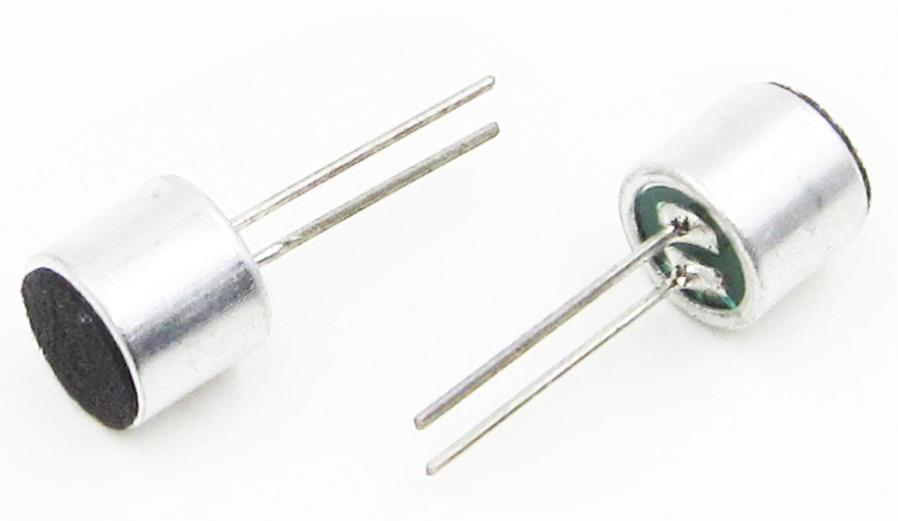
\includegraphics[height=3.5cm]{zdjecia/mic_electret.jpg}
		\subcaption{Mikrofon eletretowy}
	\end{subfigure}
	\begin{subfigure}{.45\textwidth}
		\centering
		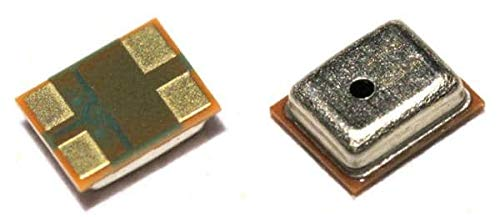
\includegraphics[height=3.5cm]{zdjecia/mic_mems.jpg}
		\subcaption{Mikrofon MEMS}
	\end{subfigure}
	\caption{\label{mikrofony} Mikrofony w różnych technologiach}
\end{figure}

Do celów projektu wybrany został mikrofon \textit{SPW2430HR5H-B} firmy \textit{Knowles}. Ponieważ jest to urządzenie on-chip, konieczne było dostosowanie projektu tak, aby płytka była maksymalnie blisko zewnętrznej ścianki obudowy. Port do akwizycji znajduje się w górnej części elementu i jest odsunięty o $ 1mm $ od dolnej części, a więc ok. $ 1mm $ od powierzchni PCB.
Jednym z głównych kryteriów wyboru była czułość. Informuje ona, jaka amplituda sygnału wyjściowego mikrofonu odpowiada danemu poziomowi ciśnienia akustycznego. W specyfikacji podawana jest jako ujemna wartość $dBV/Pa$ mierzona falą akustyczną o częstotliwości $1kHz$ i SPL $94dB$. Jednostka $dBV$ oznacza liczbę decybeli w odniesieniu do $1V$\cite{MicSens}. Stąd wzór na czułość wygląda następująco:

\begin{equation}
    Sensitivity_{dBV} = 20 \cdot log_{10}\frac{Sensitivity_{mV/Pa}}{Output_{REF}}
\end{equation}

gdzie: \\
\indent$Sensitivity_{dBV}$ - czułość w dBV/Pa \\
\indent$Sensitivity_{mV/Pa}$ - czułość w mV/Pa \\
\indent$Output_{REF}$ - wyjściowe napięcie odniesienia ($1000mV/Pa$) 

Powyższy wzór można przekształcić, aby z podanej w nocie katalogowej czułości obliczyć poziom napięcia dla danego SPL.
\begin{equation}
    Sensitivity_{mV/Pa} = 1000 \cdot 10^{\frac{Sensitivity_{dBV}}{20}}
\end{equation}

Wybrany mikrofon ma średnią czułość $-42 dbV/Pa$, a więc zgodnie ze wzorem $7,943 mV/Pa$. Stąd przy poziomie ciśnienia akustycznego $1Pa$ zmiana sygnału wyjściowego mikrofonu wyniesie $7,943 mV$. Według specyfikacji maksymalny poziom SPL to $129 dB$, czyli $56,37 Pa$. Maksymalnym napięciem wyjściowym mikrofonu powinno być więc $447,75 mV$.

Czułość mikrofonu jest zwykle odwrotnie proporcjonalna do jego maksymalnego SPL. Dlatego w projekcie słuchawek strzeleckich, które są przeznaczone do nasłuchiwania zarówno skrajnie cichych, jak i skrajnie głośnych dźwięków, zastosowanie jednego mikrofonu wymaga kompromisu między oboma parametrami. 

Rozwiązaniami w tej sytuacji byłoby zastosowanie dwóch mikrofonów o różnych czułościach lub dodanie wzmacniacza sterowanego przez oprogramowanie. Pierwsze z nich gwarantuje dobrą akwizycję wszystkich poziomów dźwięków, jednak jest wyzwaniem pod względem konstrukcyjnym, wymaga użycia większej liczby przetworników analogowo-cyfrowych i sprawnego przełączania przetwarzania przez oprogramowanie. Drugie zaś bazowałoby na mikrofonie o małej czułości i przy małych natężeniach dźwięku zwiększaniu jego amplitudy wyjściowej przez wzmacniacz sterowany potencjometrem cyfrowym. To rozwiązanie wydaje się być lepsze, choć również wymaga zaprogramowania portów mikrokontrolera tak, aby dostosowywały wzmocnienie.

W tym konkretnym przypadku problemem jest konieczność przetwarzania dźwięków o amplitudach przekraczających $140dB$
\textbf{REFERENCJA}
Znalezienie mikrofonu z takim wysokim progiem jest bardzo trudne, dlatego prawdopodobnie konieczne by było mechaniczne wyciszenie dźwięków docierających do mikrofonu, aby obniżyć odbierany poziom ciśnienia akustycznego.

Słuchawki zostały dodatkowo zaprojektowane tak, aby była możliwość podłączenia ich do radiotelefonu. Do tego celu został wybrany jeszcze jeden mikrofon montowany w elastycznej rurce przed ustami użytkownika i umożliwiający rozmowę z użyciem komunikacji radiowej. W tym przypadku jest to mikrofon elektretowy \textit{CMEJ-4622-25-L082}, ponieważ jego montaż nie wymaga padów lutowniczych. Nie było konieczne wybieranie mikrofonu o dobrym SNR, ponieważ komunikacja radiowa i tak wprowadza duże szumy. Czułość mikrofonu powinna być natomiast stosunkowo mała, ponieważ odległość od źródła dźwięku jest niewielka.